%%
%% Meta: TI nSpire Einführung
%%       Ziel: Damit die Grundoperationen damit durchgeführt werden können.
%%             Damit man sich an den Rechner gewöhnt.
%%

%% Philipp G Freimann Juli 2019 für die BBW
%% Phi BBW-Vorlage für Arbeitsblätter (LaTeX)
%% 2019 - 08 - 18

%% %% %% %%
\documentclass[twoside,12pt,a4paper]{article}%%
\usepackage[paper=a4paper,margin=17mm]{geometry}%%


%% Zentralisiert
%%\usepackage{german} %% Macht Probleme mit grafiken
\usepackage{mciteplus}

\usepackage[dvipsnames,table]{xcolor}

\usepackage{pgfplotstable}
\usepackage{tikz}
\usepackage{tkz-euclide} %% Grid

\usepackage{amsthm}
\usepackage{amsfonts} %% Zahlmengen Z, R, ...


%% THEOREMS?
\usepackage{tcolorbox}
\tcbuselibrary{theorems}
\tcbuselibrary{skins}


\usepackage{fancyhdr}
\usepackage{ngerman}
\usepackage[utf8]{inputenc}


%%\usepackage[dvips]{graphicx}

\usepackage{supertabular}
\usepackage{makeidx}  
\usepackage{ifthen} 

\usepackage{multirow}
\usepackage{listings}

%%\usepackage{color,fancyvrb,fancybox}
\usepackage{multicol}
\usepackage{lastpage}
%%\usepackage{listings}
\usepackage{pstricks}

%% bold typewriter font:
\usepackage[T1]{fontenc}
\usepackage{lmodern}

\usepackage{enumitem}
%\usepackage{enumerate}

\usepackage{float}

\usepackage{titlesec}
\usepackage{textcomp}

%% Kuchendiagramme
%%\usepackage{datapie}

%% für Aufgaben Hervorhebung
%%\usepackage[most]{tcolorbox}
%%\usepackage[standard,framed]{ntheorem}
\usepackage{framed}
\usepackage{mdframed}

%%%%%%%%%%%%%%%%%%%%
%%\usepackage[most]{tcolorbox}

\usepackage[tocindentauto]{tocstyle}

%% für accentset wedge:
\usepackage{accents}

%% Würfel
\usepackage{epsdice}

%% Einbinden von GeoGebra Bildchen:
\usetikzlibrary{shapes.geometric}
\usetikzlibrary{arrows}
\newcommand{\degre}{\ensuremath{^\circ}}

%% Hyperlinks
\usepackage{hyperref}

\hypersetup{
    colorlinks=true,
    linkcolor=blue,
    filecolor=magenta,      
    urlcolor=cyan,
    bookmarks=true,
}

%% bugtracker (part of pgfplots) should be loaded AFTER "hyperref"
%% See: https://texblog.net/hyperref/ AND https://tex.stackexchange.com/questions/16268/warning-with-footnotes-namehfootnote-xx-has-been-referenced-but-does-not-exi
\usepackage{pgfplots}
\pgfplotsset{width=10cm,compat=1.9}

%%\usepackage{fourier}  %% eg overarc (Bogenmaß)

%%%%%%%%%%%%%%%%% L A Y O U T  %%%%%%%%%%%%%%%%%%%%%%%%%%%%
%% 2020-12-27 ph. g. freimann @ bbw.ch
%%

\fancyhf{}%%

\pagestyle{fancy}%%

\renewcommand{\sectionmark}[1]{%%
  \markboth{\thesection{} \ #1}{}%%
}%%

\renewcommand{\subsectionmark}[1]{%%
  \markright{\thesubsection \ #1}%%
}%%

%% Achtung: chaptermark nur im BOOK-Style

\renewcommand{\footrulewidth}{0.4pt}

\parskip4pt
\parindent0pt

\topmargin-2.0cm
\textheight24.4cm

\renewcommand{\arraystretch}{1}%%


\newenvironment{bbwFillInTabular}{%%
%% BEGIN PART:
\renewcommand{\arraystretch}{2.1}
\begin{tabular}%%
}%% END PART:
{\end{tabular}
\renewcommand{\arraystretch}{1}%%
}%% END Environment bbwFillInTabular

%%%%%%%%%%%%%%%%%%%%%%%%%%%%%%%%%%%%%%%%%%%%%%%%%%%%%%%%%%
%%%%%%%%%%%%%%%%%% M A K R O S %%%%%%%%%%%%%%%%%%%%%%%%%%%
%%%%%%%%%%%%%%%%%%%%%%%%%%%%%%%%%%%%%%%%%%%%%%%%%%%%%%%%%%

%%%%%%%%%%%%%%%%%%%%%%%% g e n e r e l l e   M a k r o s %%%%%%%%%%%%%%%%%%%%%%%

%% Info vorab bei \newcommand
%% \newcommand{ - Kommandos können in den Parametern auch Leerzeilen
%%     enthalten
%% \newcommand*{ - Kommandos, also mit *, können jedoch in den
%%    Argumenten KEINE \par (sprich Leerzeilen} enthalten

%% 2019-07-26
%% phi@freimann.eu
%% Makros for BBW-Tex Documents
\usepackage{inputs/bbwColors}

%%%%%%%%%%%%%%%%%% I N C L U D E S   &   I N D E X  %%%%%
\graphicspath{{../img/}}
\graphicspath{{./img/}}

\newcommand*\bbwGraphicRaise[3]{\raisebox{#1}{\includegraphics[width=#2]{#3}}}%%
\newcommand*\bbwGraphic[2]{\bbwGraphicRaise{-5mm}{#1}{#2}}%%
\newcommand*\bbwCenterGraphicRaise[3]{\begin{center}\bbwGraphicRaise{#1}{#2}{#3}\end{center}}
\newcommand*\bbwCenterGraphic[2]{\bbwCenterGraphicRaise{-5mm}{#1}{#2}}%%


%% All in one Skript
\newif\ifisALLINONE
\isALLINONEfalse

%% Blended Learning
%% Insb. MatheNinja Links. Diese sind jedoch in einem anderen Kurs!
\newif\ifisBLENDED
\isBLENDEDfalse


%%%%%%%%% TRAINER Version vs. Schülerversion %%%%%%%%%%%%%
%% Bem. Kein *-Kommando, da die TRAINER-Blöcke auch leerzeilne (\par)
%% enthaltne können
\newcommand\TRAINER[1]{%%
{%%
\ifisTRAINER{\color{BlueGreen}{#1}}%%
\fi%%
}}%%  

\newcommand\TALS[1]{%
{%%
\ifisTALS{#1}%%
\fi%%
}}%

\newcommand\GESO[1]{%
{%%
\ifisGESO{#1}%%
\fi%%
}}%    

\newcommand\BLENDED[1]{%
{%%
\ifisBLENDED{#1}%%
\fi%%
}}%    

\newcommand{\noTRAINER}[1]{{\ifisTRAINER{}\else{#1}\fi}{}}%%



%%\makeatletter
%% Je nach Umgebung "environment" wird das mmPapier breiter oder
%% schmaler
%% bei itemize sollen 16.4 und bei definiton-Boxen 16.8 mm genommen
%% werden.


\usepackage{inputs/mmPapierbreiteSty}


%% Trainer "no" Dotfill
%% If no Trainer: Dotfill
\newcommand*{\TNDF}[1]{\TRAINER{#1}\noTRAINER{\dotfill{}}}%%

\newcommand*{\leserluft}{\vspace{2mm}}

%% Notiz felder 
%% Anwendung:
%% \noteField{10}  
%%  --> Notizfeld mit 10 Leerzeilen
\newcounter{DFCounter}


%%Häuschenpapier
\newcommand{\mmPapierZwei}[2]{\begin{tikzpicture}
%%  \draw[step=4mm,bbwMMFarbe,ultra thin]
%%  \draw[step=4mm,bbwMMFarbe,thick]
  \draw[step=4mm,bbwMMFarbe,line width=0.02mm]
  (0, 0) grid ({#2}, {#1});
\end{tikzpicture}}%%


%% millimeterPapier füllen bis Ende Seite
\newcommand{\mmPapierBisEndeSeite}{

\begin{tikzpicture}

\newdimen\spaceleftOnPage
\spaceleftOnPage=\dimexpr\textheight-\pagetotal-14pt\relax

\pgfmathsetmacro{\gridWidth}{\textwidth        - mod(\textwidth,      4mm)      }
\pgfmathsetmacro{\gridHeight}{\spaceleftOnPage - mod(\spaceleftOnPage,4mm) - 4mm}

\draw [step=4mm,bbwMMFarbe,line width=0.02mm] (0,0) grid (\gridWidth pt,\gridHeight pt);
\end{tikzpicture}%%
\newpage%%
}%% END Makro mmPapieBisEndeSeite


%% Standardbreite für Arbeitsblätter und das Theorieheft
%% Wird in bbwPruefung.sty überschrieben, da dort schmaler
\def\defaultTextBreite{17.6}
\def\unitCMWhatElse{cm}%% wird als Breitenangabe für den nächsten command verwendet

%% Verwendung: \bbwCenterGraphic{\defaultTextBreite}{«img url»}
\def\defaultTextBreiteCM{\defaultTextBreite\unitCMWhatElse}
\newcommand{\mmPapier}[1]{\mmPapierZwei{#1}{\defaultTextBreite}}


%% Notizen Berechungen auf Prüfungsblättern
\newcommand{\platzFuerBerechnungen}[1]{\noTRAINER{

Notizen / Berechnungen:

\mmPapier{#1}}}%% end platzFuerBerechnungen

\newcommand{\platzFuerBerechnungenBisEndeSeite}[1]{\noTRAINER{

Notizen / Berechnungen:

\mmPapierBisEndeSeite}}%% end platzFuerBerechnungen



\newcommand{\platzFuerBerechnungenOhneText}[1]{\noTRAINER{

\mmPapier{#1}}}

%% Die Abkürzung z.\,B. von «Zum Beispiel» hat einen verkleinerten Abstand.
\newcommand*\zB{%
z.\,B.
}

%%
%% Auf der Titelseite steht entweder GESO oder TALS.
%% Dies wird gleich mit der Fußnote angegeben.
%% Dieses Kommando sollte im Kommando «\untertitel» eingesetzt werden.
%%
\newcommand*\ausrichtungAufTitelseite{%
\ifisTALS{TALS\noTRAINER{\footnote{TALS «Technik, Architektur und Life Sciences
(Laboranten)»: Ausrichtung technisches Profil}}}%%
\fi%%
\ifisGESO{GESO\noTRAINER{\footnote{GESO: Ausrichtung \textbf{Ge}sundheit und \textbf{So}ziales}}}%%
\fi}%%

%%%%%%%%%%%%%%%%%%%%%% B B W - M a t h e   F a r b c o d e s  %%%%%%%%%%%%%%%%%%%%%%%%%%%%%%555

\newcommand{\rezeptFarbe}{rezeptFarbe}
\newcommand{\definitionFarbe}{definitionFarbe}
\newcommand{\gesetzFarbe}{gesetzFarbe}
\newcommand{\beispielFarbe}{beispielFarbe}
\newcommand{\bemerkungFarbe}{bemerkungFarbe}

%% Falls gewünscht übersteuren
%  \definecolor{xyz}{HTML}{eeff66}
%  \renewcommand{\beispielFarbe}{xyz}
%

%% Theorem-Styles
\newcommand\theoremlayoutdefinition[4]{\newtcbtheorem[number within=section]{#1}{#2}%
   {theorem style=plain,enhanced,colframe=#3!20!white,colback=#3!20!white,
     coltitle=#3!60!black,fonttitle=\upshape\bfseries,
     %%fontupper=\itshape,
    %%drop fuzzy shadow=blue!50!black!50!white,
    terminator sign={:},
    borderline north={0.5mm}{0pt}{#3}, borderline south={0.5mm}{0pt}{#3}
}{#4}}



%% Farben für rezept, definition und gesetz von Marthale übernommen.
%% Verwendung mit * unterbindet die Nummerierung \begin{gesetz*}{Blah}{xy} ...\end {gesetz*}
\theoremlayoutdefinition{rezept}{Rezept}{\rezeptFarbe}{R}
\theoremlayoutdefinition{definition}{Definition}{\definitionFarbe}{D}
\theoremlayoutdefinition{gesetz}{Gesetz}{\gesetzFarbe}{G}%% was green
\theoremlayoutdefinition{beispiel}{Beispiel}{\beispielFarbe}{B}
\theoremlayoutdefinition{bemerkung}{Bemerkung}{\bemerkungFarbe}{M}

%%
%% Force a blank page, when \newpage does not work
%%
\def\blankpage{%
	\clearpage%
	\null%
	\clearpage}%%

\newcommand{\Lueckentext}[1]{\,\,\noTRAINER{\dotfill}\TRAINER{#1}}


\newcommand{\LoesungsRaumCM}[2]{\,\,\noTRAINER{\underline{\hspace{#1}}}\TRAINER{#2}}

\newcommand{\LoesungsRaum}[1]{\LoesungsRaumCM{30mm}{#1}}
\newcommand{\LoesungsRaumKurz}[1]{\LoesungsRaumCM{15mm}{#1}}
\newcommand{\LoesungsRaumLang}[1]{\LoesungsRaumCM{45mm}{#1}}


%% TI nSpire
\def\tinspire{\texttt{TI-nSpire}}

%% TI 30 Pro Mathprint Button Images
\def\tiprobuttonbreite{10mm}
\def\nspirebuttonbreite{8.6mm}

%%\def\sec{\raisebox{-2mm}{\includegraphics[width=\buttonbreite{}]{img/tiprobuttonimages/2nd.png}}}
\newcommand{\tiprobutton}[1]{\raisebox{-2mm}{\mbox{\,\includegraphics[width=\tiprobuttonbreite{}]{img/tiprobuttonimages/#1.png}\,}}}

\newcommand{\nspirebutton}[1]{\raisebox{-2mm}{\mbox{\,\includegraphics[width=\nspirebuttonbreite{}]{img/nspirebuttonimages/#1.png}\,}}}

%% Counter  für Aufgaben
%% Bei jedem Part wird die Aufgabennummer zurückgesetz auf 1
\newcommand{\bbwPartID}{AA1}
\newcommand{\bbwAufgabenBlockID}{}
\newcounter{bbwAufgabenNummerCounter}[part]
\setcounter{bbwAufgabenNummerCounter}{1}
\newcommand{\bbwAufgabenNummer}{\arabic{bbwAufgabenNummerCounter}}
\newcommand{\nextBbwAufgabenNummer}{\stepcounter{bbwAufgabenNummerCounter}}
\newcommand{\aufgSubLabel}{{\color{blue}\bbwAufgabenNummer. \alph*)}}

%% Benutze außerhalb der bbwAufgabenblöcke folgendes Kommando, um an die
%% nächste Aufgabennummer zu kommen. Dies z. B. wenn ein längerer Text vor der Aufgabe steht,
%% der auch schon diese Bezeichnung erhalten sollte
\newcommand{\bbwActAufgabenNr}{{\color{blue}\bbwAufgabenNummer. {\small[\bbwAufgabenBlockID]}}}


\newenvironment{bbwAufgabenBlock}{%% Begin environment Part:

\bbwActAufgabenNr{}
%%{\color{blue}\bbwAufgabenNummer. {\small[\bbwAufgabenBlockID]}}
\begin{enumerate}[label=\aufgSubLabel]
}%% Ende der Präambel
{%% END Part:
\end{enumerate}
\nextBbwAufgabenNummer
}%% END environment bbwAufgabenBlock

%%%%%%%%%%%%%%%%%%%%%%%%%%%%

%% Weblinks und Mathe Ninja Links

\newcommand{\weblink}[2]{\href{#2}{#1}}

\newcommand{\olatBBWLogo}{
\includegraphics[width=15mm]{logos/traube.pdf}}%%
\newcommand{\externerLinkEPS}{
\includegraphics[width=15mm]{logos/extLink.pdf}}%%
\newcommand{\youtubeLogo}{\includegraphics[width=15mm]{logos/youtube.png}}%%


%%
%% #1: Text
%% #2: URL
%% #3: Aufgabennummern
%% #4: optional weitere Logos oder leer lassen {}
\newcommand{\externalLink}[4]{%%
\begin{tabular}{|lp{111mm}|}\hline%%
\multicolumn{2}{|p{172mm}|}{\cellcolor{aufgabenFarbe}#3}\\
\weblink{\raisebox{-5mm}{\externerLinkEPS{}}}{#2} {#4}  & \weblink{#1}{#2}\\\hline
\multicolumn{2}{|p{172mm}|}{\weblink{#2}{#2}}\\\hline
\end{tabular}%%
\vspace{1mm}
}%% END Command externalLink

%% #1: URL
%% #2: Text
\newcommand{\youtubeLink}[2]{%%
\externalLink{#2}{#1}{Youtube}{\raisebox{-5mm}{\youtubeLogo{}}}
}%%

%%
%% #1: Typ-Logo (eg. LOGO auf MatheNinja)
%% #2: Typ-Name (eg «Mathe Ninja»
%% #3: URL
%% #4: Aufgaben Name
\newcommand{\olatLink}[4]{%%
\begin{tabular}{|lp{111mm}|}\hline%%
\multicolumn{2}{|p{172mm}|}{\cellcolor{aufgabenFarbe}#4}\\
\weblink{\raisebox{-5mm}{\externerLinkEPS{}}}{#3} \weblink{\raisebox{-5mm}{\olatBBWLogo}}{#3} \weblink{#1}{#3}& \weblink{#2}{#3}\\\hline
\end{tabular}%%
\vspace{1mm}
}%% END Command olatLink


%\newcommand{\olatLOGOLink}[3]{%%
%\begin{tabular}{|lp{111mm}|}\hline%%
%\weblink{\raisebox{-5mm}{\olatBBWLogo{}}}{#2} & \weblink{#1}{#2}\\
%\multicolumn{2}{|p{172mm}|}{\cellcolor{aufgabenFarbe}#3}\\\hline
%\end{tabular}%%
%}%% END Command olatLOGOLink

%% Use:
%% \olatLinkArbeitsblatt{Kapitel/Arbeitsblattname «[ID]»}{«URL»}{Aufgabennummern}
\newcommand{\olatLinkArbeitsblatt}[3]{\olatLink{\raisebox{-6mm}{
\includegraphics[width=12mm]{logos/seite.pdf}}}{Arbeitsblatt: #1}{#2}{#3}}%%

%% #1: Text
%% #2: URL
\newcommand{\olatLinkPruefung}[2]{\olatLink{\raisebox{-6mm}{
\includegraphics[width=15mm]{logos/test.pdf}}}{Online Test}{#2}{#1}}%%


%%
%% use:
%% \matheNinjaLink{Beschreibung}{URL}
\newcommand{\matheNinjaLink}[2]{\olatLink{\raisebox{-6mm}{\includegraphics[width=17mm]{img/matheninja/matheninja.jpg}}}{Mathe Ninja!}{#2}{#1}}%%


%% Use
%% \olatLinkGESOKompendium{Kapitel}{Seite/Seiteff}{Aufgabe(n)}
\newcommand{\olatLinkGESOKompendium}[3]{%%
\GESO{%%
\olatLink{{\Huge K}}{Kompendium}{https://olat.bbw.ch/auth/RepositoryEntry/572162163/CourseNode/106029172671728}{Kapitel #1; Seite #2; Aufg. #3}%%
}%% END GESO
}%%


%% Use \olatLinkTALSStrukturaufgabenSPF{Kapitel}{Seite/Seiteff}{Aufgabe(n)}
\newcommand{\olatLinkTALSStrukturaufgabenSPF}[3]{%%
\TALS{%%
\olatLink{{\Huge S}}{Strukturaufgaben}{https://olat.bbw.ch/auth/RepositoryEntry/572162090/CourseNode/102901174299246}{Kapitel #1; Seite #2; Aufgaben #3}%%
}%% END GESO
}%%

%%\newcommand{\olatLinkTALtfSStrukturaufgabenGLF}[1]{\olatLOGOLink{Strukturaufgaben Grundlagenfach}{https://olat.bbw.ch/auth/RepositoryEntry/572162090/CourseNode/102901174291476}{#1}}


%%\newcommand{\matheNinjaLink}[2]{%%
%%\begin{tabular}{cc}%%
%% \raisebox{-1cm}{\includegraphics[height=2cm]{img/matheninja/turtle.png}}& \href{#2}{MatheNinja: #1}\\%%
%% \end{tabular}%%
%%}%% End Command  \matheNinjaLink



%% AadB = Aufgaben aus dem Buch
%% 1. Parameter: Seitenzahl
%% 2. Parameter: Aufgabennummern.
%% bsp  \TALSAadB{38-39}{101a-101c, 102 und 103}

%%\newcommand*{\maturaAufgaben}[1]{\begin{mdframed}[backgroundcolor=maturaAufgabenFarbe!10]{#1}\end{mdframed}}

\newcommand*{\aadBTxt}{Aufgaben aus dem Buch}


%%
% Generell Aufgaben aus einem Lehrbuch
% #1: cite auf das Lehrbuch (z. B. frommenwiler17alg)
% #2: Seitennummer oder Seitennumerff
% #3: aufgabennummer(n)
\newcommand*{\AadB}[3]{%%
\aufgabenFarbe{\noindent{\aadBTxt \cite{#1}: Seite {#2} Nr. {#3}}}%%
}%%

%%\newcommand*{\AdbBAlgebra}[2]{\AadB{marthaler21alg}{#1}{#2}}%%

\newcommand*{\TALSAadBFWA}[2]{\ifisTALS{\AadB{frommenwiler17alg}{#1}{#2}}\fi}%%
\newcommand*{\TALSAadBMTA}[2]{\ifisTALS{\AadB{marthaler21alg}{#1}{#2}}\fi}%%
\newcommand*{\TALSAadBFWG}[2]{\ifisTALS{\AadB{frommenwiler18geom}{#1}{#2}}\fi}%%
\newcommand*{\TALSAadBMTG}[2]{\ifisTALS{\AadB{marthaler20geom}{#1}{#2}}\fi}%%

%% GESO hat (noch) keine Geometrie
\newcommand*{\GESOAadBMTA}[2]{\ifisGESO{\AadB{marthaler21alg}{#1}{#2}}\fi}%%

\newcommand*{\AadBMTA}[2]{\AadB{marthaler21alg}{#1}{#2}}
\newcommand*{\AadBMTG}[2]{\AadB{marthaler20geom}{#1}{#2}}

%%
% Generell Theorie aus einem Lehrbuch
% #1: cite auf das Lehrbuch (z. B. frommenwiler17alg)
% #2: Seitennummer oder Seitennumerff
% #3: KapitelNummer
\newcommand*{\TadB}[3]{%%
\aufgabenFarbe{\noindent{Theorie \cite{#1}: Seite {#2} Nr. {#3}}}%%
}%%

\newcommand*{\TALSTadBFWA}[2]{\ifisTALS{\TadB{frommenwiler17alg}{#1}{#2}}\fi}%%
\newcommand*{\TALSTadBMTA}[2]{\ifisTALS{\TadB{marthaler21alg}{#1}{#2}}\fi}%%
\newcommand*{\TALSTadBFWG}[2]{\ifisTALS{\TadB{frommenwiler18geom}{#1}{#2}}\fi}%%
\newcommand*{\TALSTadBMTG}[2]{\ifisTALS{\TadB{marthaler20geom}{#1}{#2}}\fi}%%

%% GESO hat (noch) keine Geometrie
\newcommand*{\GESOTadBMTA}[2]{\ifisGESO{\TadB{marthaler21alg}{#1}{#2}}\fi}%%
\newcommand*{\TadBMTA}[2]{\TadB{marthaler21alg}{#1}{#2}}
\newcommand*{\TadBMTG}[2]{\TadB{marthaler20geom}{#1}{#2}}


%% Referenzen auf Labels
%% AllInOne ist wichtig, denn einige Referenzen funkitionieren nicht
%% in den Themen-Skripts, sondern lediglich in den gesamten Jahres-Skripts.
\newcommand*\totalref[1]{\ifisALLINONE{ (s.\kern 0.22em{}Kap. \ref{#1}
    auf Seite \pageref{#1}) }\else{}\fi{}}%%
\newcommand*\totalrefanhang[1]{ (s.\kern 0.22em{}Kap. \ref{#1}
    auf Seite \pageref{#1}) }%%

%% Short version
\newcommand*\totalrefs[1]{\ifisALLINONE{ Kap. \ref{#1} auf Seite
\pageref{#1} }\else{}\fi{}}%%
%%\newcommand*\aufgabenref[1]{(s\kern 0.22em{}Aufg. \ref{#1} auf Seite \pageref{#1})}

%%%%%%%%%%%%%%%%%%%%%%%%%%%%%%%%%%% BBW Makros %%%%%%%%%%%%%%%%%%%%%%%%%%%%%


%% Philipp G Freimann Juli 2019 für die BBW
%% Phi BBW-Vorlage für Mathematische Dokumente (LaTeX)
%% 2019 - 07 - 11
%%%%%%%%%%%%%%%%%%%%%%%%%%% M a t h e   M a k r o s %%%%%%%%%%%%%%%%%%%%%%%%%%%%%5

\usetikzlibrary{arrows.meta}

%% Kleine Symbole über anderen. Z. B. "?" über einem
%% Gleichheitszeichen:
%% Use \ueberMini{=}{?} um ein kleines Fragezeichen über ein
%% Gleichheitsszeichen zu schreiben.
\newcommand{\ueberMini}[2]{ \mathrel{\stackrel{\makebox[0pt]{\mbox{\normalfont\tiny #2}}}{#1}} }

%% Gleichungssystem mit zwei Zeilen und vier Einträgen (je zwei links
%% bzw. rechts).
\def\gleichungZZ#1#2#3#4{%%
  $$\left|
  \begin{array}{rcl}
    {#1} &=& {#2}\\
    {#3} &=& {#4}
    \end{array}\right|$$}%%

\def\gleichungDD#1#2#3#4#5#6{%%
  $$\left|
  \begin{array}{rcl}
    {#1} &=& {#2}\\
    {#3} &=& {#4}\\
    {#5} &=& {#6}\\
    \end{array}\right|$$}%%

%% Entspricht-Symbol
%%\usepackage{accents}
\newcommand{\hatset}[1]{\accentset{\wedge}{#1}}
\newcommand{\entspricht}{\,\,\hatset{=}\,\,}
\newcommand*\mittelwert[1]{\bar{#1}}
\newcommand*\mediantilde[1]{\widetilde{#1}}

%%
%% Graphiken mit tikz: BBW-Mathe-akros
%%
\tikzset{bbwgrid/.style={help lines,color=cyan!18, step=0.5cm}}

\newcommand{\bbwGridPart}[4]{
 % grid:
 \draw[bbwgrid] (#1,#3) grid (#2,#4);

 % axes
 \draw[thick] (#1,0) -- (#2,0);
 \draw[thick] (0,#3) -- (0,#4);
 \foreach \x in {#1, ..., -1}  \draw (\x cm, 2pt) -- (\x cm, -2pt)  node[anchor=north]{$\x$};
 \foreach \x in {1, ..., #2}   \draw (\x cm, 2pt) -- (\x cm, -2pt)  node[anchor=north]{$\x$};
 \foreach \y in {#3, ..., -1}  \draw (-2pt, \y cm) -- (2pt, \y cm)  node[anchor=east]{$\y\,\,$};
 \foreach \y in {1, ..., #4}   \draw (-2pt, \y cm) -- (2pt, \y cm)  node[anchor=east]{$\y\,\,$};
 \draw[->,thick] (#2,0) -- ({#2+0.5},0) node[anchor=west]{$x$};
 \draw[->,thick] (0,#4) -- (0,{#4+0.5}) node[anchor=south]{$y$};
}


%% A function within a Grid (without painting the grid)
%% #1: funciton eg 2*\x  (x has to be backquoted)
%% #2: Domain eg. -1:2.5
%% #3: colour eg red
\newcommand{\bbwFuncC}[3]{\draw[domain=#2,smooth,samples=200,variable=\x,#3] plot ({\x},{#1});
}
%% A function within a Grid (without painting the grid)
\newcommand{\bbwFunc}[2]{\bbwFuncC{#1}{#2}{blue}}

%% Declare a function-plot
%% xmin,xmax,ymin,ymax,fct,domain(x-min, x-max)
%% example: \bbwFunction{-4}{3}{-2}{5}{-\x*\x- \x + 4.5}{-3:2}
\newcommand{\bbwFunction}[6]{\begin{tikzpicture}
\bbwGridPart{#1}{#2}{#3}{#4}
 \bbwFunc{#5}{#6}
%% \draw[domain=#6,smooth,samples=200,variable=\x,blue] plot ({\x},{#5});
\end{tikzpicture}}
%% a whole graph having a coordinate-system #1-#4 and any tizpicture content #5:
\newcommand{\bbwGraph}[5]{\begin{tikzpicture}\bbwGridPart{#1}{#2}{#3}{#4}#5\end{tikzpicture}}

%% Dots and lines:
%% Dot example: \bbwDot{-1,2}{red}{east}{A}
\newcommand{\bbwDot}[4]{\filldraw[color=#2!60, fill=#2!5, thick](#1) circle(0.05) node[anchor=#3]{$#4$};}

%% Line example: \bbwLine{-1,0}{2,3}{red}
\newcommand{\bbwLine}[3]{\draw[thick,color=#3] (#1)--(#2);}

\newcommand{\bbwArrow}[3]{\draw[thick,color=#3,->] (#1)--(#2);}


%% Draw a single letter or small text
% #1: Position eg  4,4
% #2: letter eg f or blah
% #3: colour
\newcommand{\bbwLetter}[3]{\draw[color=#3](#1) node{$#2$};}

%%% ABC-Formel
%% usage \abcd{<a>}{<b>}{<c>}
%% example usage: \abcd{b}{5}{\sqrt{4}}
\newcommand{\abcd}[3]{$\frac{-(#2)\pm\sqrt{(#2)^2 - 4\cdot{}(#1)\cdot{}(#3)}}{2\cdot{}(#1)}$}



%% Trigonometrische Koordinatensysteme
%% Alle heißen "trigsysS" wobei da S einer der folgenden Sub-Systeme
%% bezeichnet:
%%  A  phi von  0 ... 360
%%     y   von -3 ...   3
%%
%%  B  phi von  0 ... 360
%%     y   von -1 ...   1
%%
%%  C  phi von  -270 ... 450
%%     y   von    -2 ...   2
%%
%%  D  phi von  -270 ... 450
%%     y   von    -1 ...   1
%%

\newcommand{\trigsysA}{
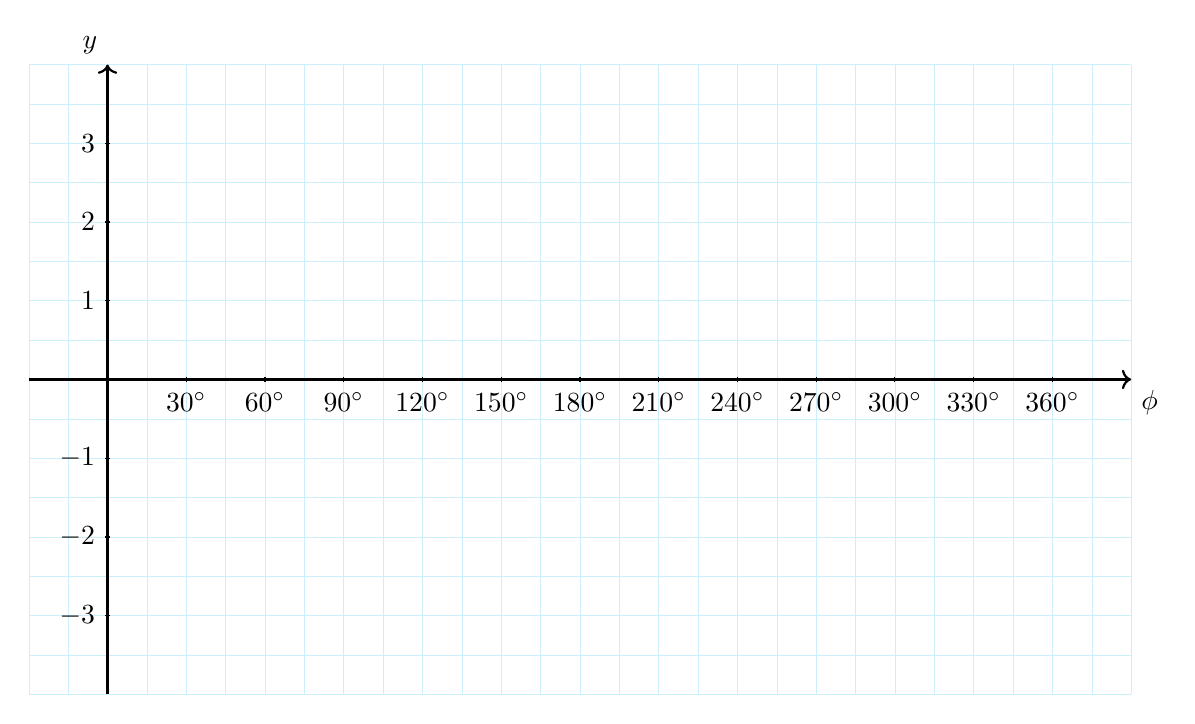
\begin{tikzpicture}
\draw[step = 0.5 cm, cyan!20 , very thin] (-1, -4) grid ( 13, 4);
\draw[thick, ->] (-1,0) -- (13,0) node[anchor = north west] {$\phi$};
\draw[thick, ->] (0,-4) -- (0,4) node[anchor = south east] {$y$};

\foreach \x [evaluate=\x as \degree using int(\x*30)] in {1,...,12}{ 
   \draw (\x cm, 1pt) -- (\x cm, -1pt) node[anchor = north] {$\degree^\circ$};
   }
\foreach \y in {-3,-2,-1,1,2,3}
   \draw (1pt, \y cm) -- (-1pt, \y cm) node[anchor = east] {$\y$};
\end{tikzpicture}}%% END Definition

\newcommand{\trigsysB}{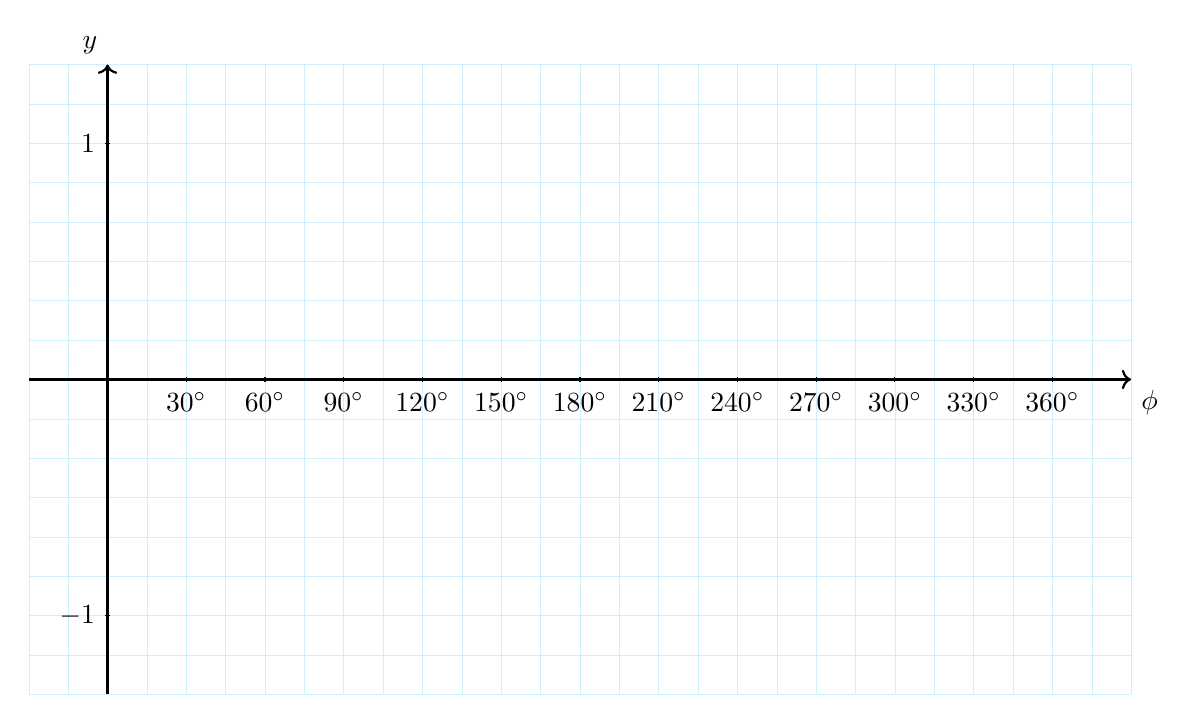
\begin{tikzpicture}\draw[step = 0.5 cm, cyan!20 , very thin] (-1, -4) grid ( 13, 4);
\draw[thick, ->] (-1,0) -- (13,0) node[anchor = north west] {$\phi$};
\draw[thick, ->] (0,-4) -- (0,4) node[anchor = south east] {$y$};

\foreach \x [evaluate=\x as \degree using int(\x*30)] in {1,...,12}{ 
   \draw (\x cm, 1pt) -- (\x cm, -1pt) node[anchor = north] {$\degree^\circ$};
   }
\foreach \y in {-1,1}
   \draw (1pt, \y *3cm) -- (-1pt, \y *3cm) node[anchor = east] {$\y$};

\end{tikzpicture}}%% END Definition

\newcommand{\trigsysC}{
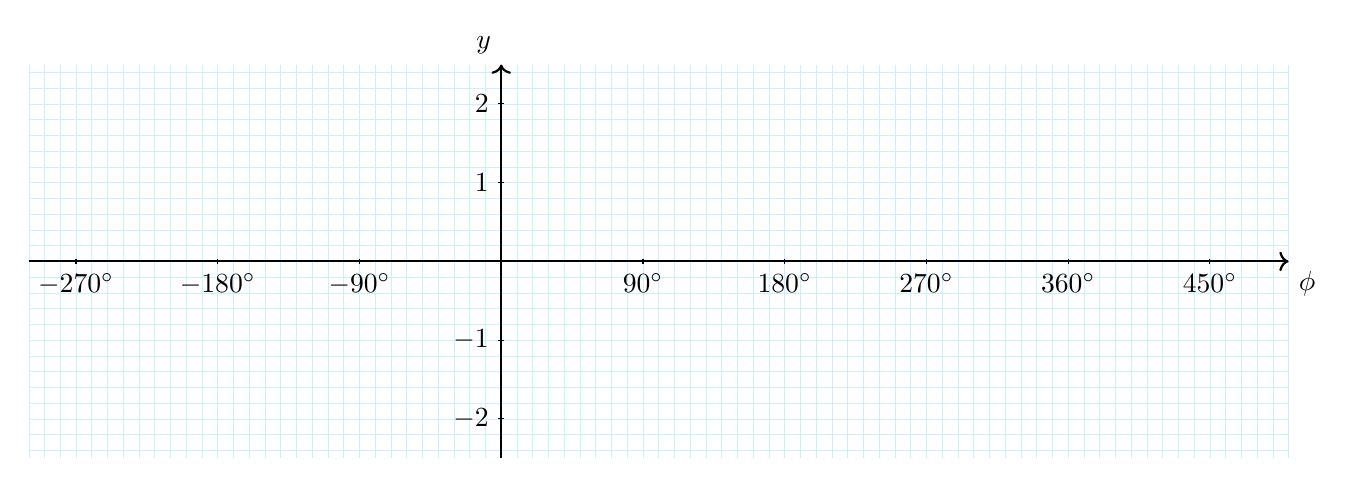
\begin{tikzpicture}
\draw[step = 0.2 cm, very thin, cyan!20] (-6, -2.5) grid ( 10, 2.5);
\draw[thick, ->] (-6,0) -- (10,0) node[anchor = north west] {$\phi$};
\draw[thick, ->] (0,-2.5) -- (0,2.5) node[anchor = south east] {$y$};

\foreach \x [evaluate=\x as \degree using int(\x*90)] in {-3,-2,-1,1,2,3,4,5}{ 
   \draw (\x *18mm, 1pt) -- (\x * 18mm, -1pt) node[anchor = north] {$\degree^\circ$};
   }
   
\foreach \y in {-2,-1,1,2}
   \draw (1pt, \y cm) -- (-1pt, \y cm) node[anchor = east] {$\y$};
\end{tikzpicture}}%% END Definition

\newcommand{\trigsysD}{
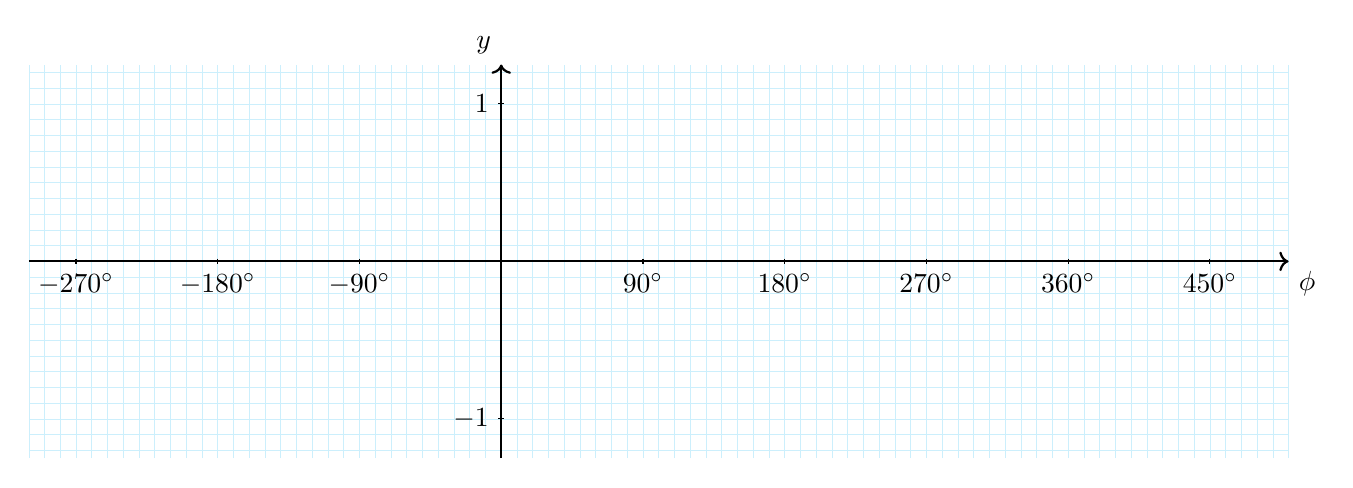
\begin{tikzpicture}
\draw[step = 0.2 cm, very thin, cyan!20] (-6, -2.5) grid ( 10, 2.5);
\draw[thick, ->] (-6,0) -- (10,0) node[anchor = north west] {$\phi$};
\draw[thick, ->] (0,-2.5) -- (0,2.5) node[anchor = south east] {$y$};

\foreach \x [evaluate=\x as \degree using int(\x*90)] in {-3,-2,-1,1,2,3,4,5}{ 
   \draw (\x *18mm, 1pt) -- (\x * 18mm, -1pt) node[anchor = north] {$\degree^\circ$};
   }
   
\foreach \y in {-1,1}
   \draw (1pt, \y *2cm) -- (-1pt, \y *2cm) node[anchor = east] {$\y$};
\end{tikzpicture}}%% END Definition


\newcommand{\trigsysDsin}{
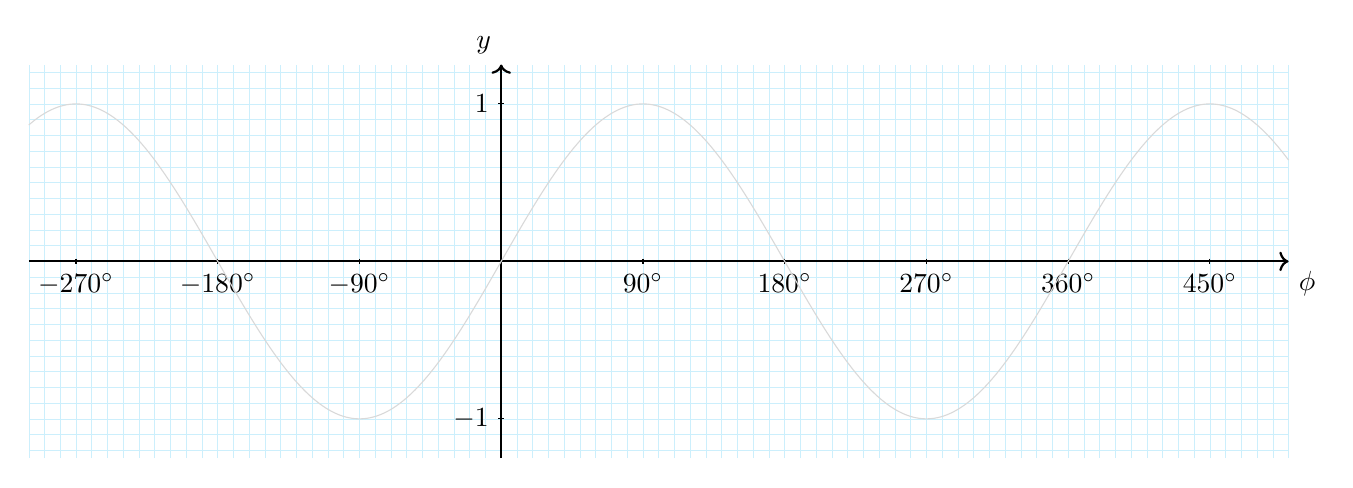
\begin{tikzpicture}
\draw[step = 0.2 cm, very thin, cyan!20] (-6, -2.5) grid ( 10, 2.5);
\draw[thick, ->] (-6,0) -- (10,0) node[anchor = north west] {$\phi$};
\draw[thick, ->] (0,-2.5) -- (0,2.5) node[anchor = south east] {$y$};

\foreach \x [evaluate=\x as \degree using int(\x*90)] in {-3,-2,-1,1,2,3,4,5}{ 
   \draw (\x *18mm, 1pt) -- (\x * 18mm, -1pt) node[anchor = north] {$\degree^\circ$};
   }
   
\foreach \y in {-1,1}
   \draw (1pt, \y *2cm) -- (-1pt, \y *2cm) node[anchor = east] {$\y$};

\draw[domain=-6:10,smooth,samples=200,variable=\x,gray!30] plot ({\x},{2*sin(\x*50)});
\end{tikzpicture}}%% END Definition

\newcommand{\trigsysDcos}{
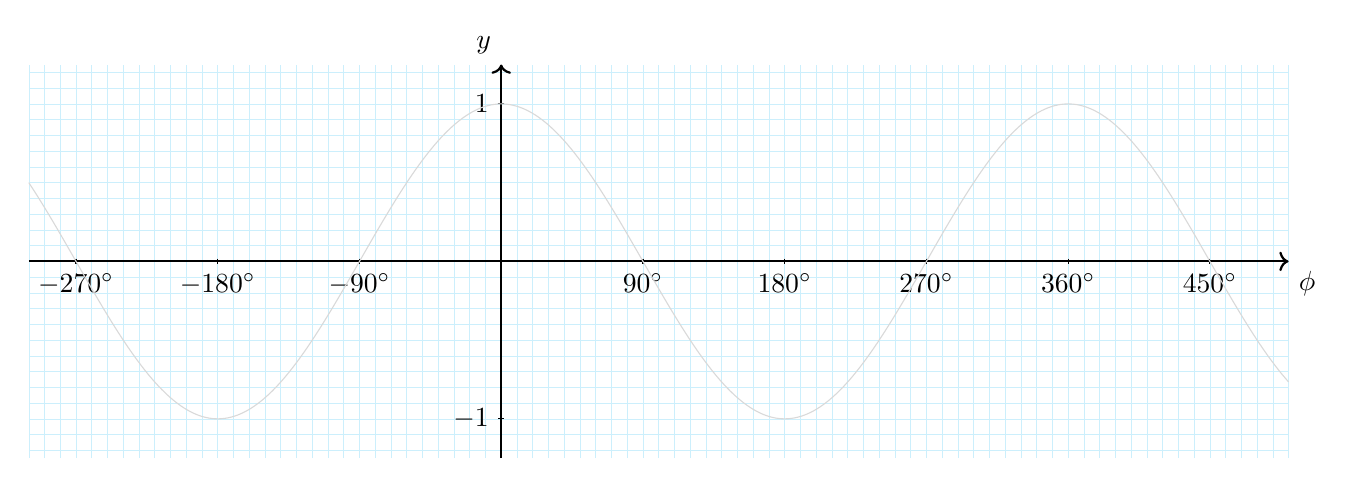
\begin{tikzpicture}
\draw[step = 0.2 cm, very thin, cyan!20] (-6, -2.5) grid ( 10, 2.5);
\draw[thick, ->] (-6,0) -- (10,0) node[anchor = north west] {$\phi$};
\draw[thick, ->] (0,-2.5) -- (0,2.5) node[anchor = south east] {$y$};

\foreach \x [evaluate=\x as \degree using int(\x*90)] in {-3,-2,-1,1,2,3,4,5}{ 
   \draw (\x *18mm, 1pt) -- (\x * 18mm, -1pt) node[anchor = north] {$\degree^\circ$};
   }
   
\foreach \y in {-1,1}
   \draw (1pt, \y *2cm) -- (-1pt, \y *2cm) node[anchor = east] {$\y$};

\draw[domain=-6:10,smooth,samples=200,variable=\x,gray!30] plot ({\x},{2*cos(\x*50)});
\end{tikzpicture}}%% END Definition


%%

\usepackage{bbwLayoutPageSty}


%%%%%%%%%%%%%%%  H E A D E R   &   F O O T E R %%%%%%%%%%%%%%%%%%%%
%% Headers
\fancyhf[HL]{\makebox{\includegraphics[width=30mm]{logos/bbw.pdf}}}%%
\fancyhf[HC]{\metaHeaderLine{}}%%
\fancyhf[FR]{\tiny{\shortAuthor{} (\today{})}}%%

\newcommand{\arbeitsblattHeader}{%%
  \begin{center}%%
    {\Large \fontfamily{qhv}\selectfont \arbeitsblattTitel{}}%%
\end{center}}%%


%%%%%%%%%%%%%%%%%%%%%%%%%%%%%%%%%%%%%%%%%%%%%%%%%%%%%%%%%%%%%%%%%%

\usepackage{amssymb} %% für \blacktriangleright
\renewcommand{\metaHeaderLine}{Lineare Funktionen}
\renewcommand{\arbeitsblattTitel}{\metaHeaderLine{} Arbeitsblatt (V 2.0)}

\begin{document}%%
\arbeitsblattHeader{}

\title{Aufgaben Funktionsbegriff}

\section{Darstellung}
\subsection{Wertetabelle und Graph}
Gegeben ist die Funktion $f$:
$$y=\frac32x-5$$


a) Erstellen Sie eine Wertetabelle für $f$:

\TRAINER{%%
\begin{tabular}{|c|c|c|c|c|c|c|c|c|c|c|}\hline
$-4$ & $-3$ & $-2$ & $-1$ & $0$ & $1$ & $2$ & $3$ & $4$ & $5$ & $6$\\\hline%%
$-11$ & $-9.5$ & $-8$ & $-6.5$ & $-5$ & $-3.5$ & $-2$ & $-0.5$ & $1$ & $2.5$ & $4$\\\hline%%
\end{tabular} 
}%% end TRAINER
\noTRAINER{%%
\begin{tabular}{|c|c|c|c|c|c|c|c|c|c|c|}
$-4$ & $-3$ & $-2$ & $-1$ & $0$ & $1$ & $2$ & $3$ & $4$ & $5$ & $6$\\\hline
 \hspace{7mm} & \hspace{7mm} & \hspace{7mm} & \hspace{7mm} &\hspace{7mm} &\hspace{7mm} &\hspace{7mm} &\hspace{7mm} &\hspace{7mm} &\hspace{7mm} &\hspace{7mm}\,\,\,\,%%
\end{tabular} 
}%% end noTRANIER

b) Zeichnen Sie den Graphen von $f$ ins folgende
Koordinatensystem; natürlich nur im passenden Bereich (Tipps:
Taschenrechner / Grundform):

\bbwGraph{-2}{6}{-7}{2}{%%
\TRAINER{\bbwFunc{\x / 2 * 3 - 5}{-1:4}}
}%% end bbwGraph

c) Geben Sie die beiden Schnittpunkte mit den Achsen an:
$$S_{y\text{Achse}} = \LoesungsRaum{(0|-5)}
\text{ und }
S_{x\text{-Achse}} = \LoesungsRaum{\left(\frac{10}3 \middle| 0\right)}$$
\newpage

\subsection{Skizzieren}
Skizzieren Sie die folgenden Funktionen $f_1$ bis $f_6$:

$f_1$: $y=2x+3$

\bbwGraph{-4}{5}{-3}{5}{
\TRAINER{\bbwFunc{2*\x + 3}{-3:1}}
}


$f_2$: $y=\frac12x-1$

\bbwGraph{-4}{5}{-3}{1}{
\TRAINER{\bbwFunc{0.5*\x  - 1}{-3:4}}
}
\newpage


$f_3$: $y=-x+1.5$

\bbwGraph{-4}{5}{-3}{5}{
\TRAINER{\bbwFunc{-\x  +1.5}{-3:4}}
}



$f_4$: $y=\frac23x-3$

\bbwGraph{-4}{6}{-5}{2}{
\TRAINER{\bbwFunc{\x*2/3 -3}{-3:5}}
}
\newpage


$f_5$: $2x=2y-4$ \TRAINER{$\Longrightarrow  y=x+2$}

\bbwGraph{-5}{5}{-2}{5}{
\TRAINER{\bbwFunc{\x+2}{-4:3}}
}



$f_6$: $\frac{2-x}3 = \frac{y-x}6$ \TRAINER{$\Longrightarrow  y=-x+4$}

\bbwGraph{-3}{5}{-2}{6.5}{
\TRAINER{\bbwFunc{-\x  +4}{-2:5}}
}
\newpage

\section{$y$-Achsenabschnitt (= Ordinatenabschnitt)}

\subsection{$y$-Achsenabschnitt rechnen}

Geben Sie jeweils den $y$-Achsenabschnitt an:

a) $y=3x-2$ $\Longrightarrow$ $y$-Achsenabschnitt =
$\LoesungsRaum{-2}$

\noTRAINER{\mmPapier{2.4}}

b) $y=4x+\frac12$ $\Longrightarrow$ $y$-Achsenabschnitt =
$\LoesungsRaum{\frac12}$

\noTRAINER{\mmPapier{3.2}}

c) $2(x+y+1) = y-4x+3$ $\Longrightarrow$ $y$-Achsenabschnitt =
$\LoesungsRaum{1}$

\TNTeop{
Umformen in Grundform:
$$2(x+y+1) = y-4x+3$$
$$2x+2y+2 = y-4x+3$$
$$2x+2y-1 = y-4x$$
$$6x+2y-1 = y$$
$$6x+y-1 = 0$$
$$6x+y= 1$$
$$y= -6x + 1$$
}
%% implicit: \newpage

\subsection{Funktionsgleichung finden}
Die Funktion $y=3x+b$ geht durch den Punkt $(0|7)$.
Berechnen Sie den Parameter $b$ oder mit anderen Worten: Geben Sie die
Funktionsgleichung an:

\TNT{4.8}{$$y=3x+7$$ denn $7$ ist als $y$-Achsenabschnitt gegeben.}
\newpage

\section{Steigung}

\subsection{Steigung von Strecken}
Geben Sie die Steigungen der folgenden Strecken an:

\bbwGraph{-8}{7}{-6}{6}{%
\bbwStrecke{ 2, 3}{ 6, 5}{ 4  , 4.5}{a)}{blue}
\bbwStrecke{-6, 4}{-3, 3}{-4.5,4}{b)}{orange}
\bbwStrecke{-7,-4}{-4,-4}{-5.5,-4.5}{c)}{green}
\bbwStrecke{-3,-2}{ 2,-5}{ 1  ,-4  }{d)}{black}
\bbwStrecke{ 0,-1}{ 4, 2}{ 2  , 1  }{e)}{pink}
\bbwStrecke{ 4,-3}{ 4,-5}{ 4.5,-4  }{f)}{ForestGreen}
}%% end BBW Graph

Lösungen:

\TNTeop{
a) $\frac12$; b) $-\frac13$; c) $0$; d) $-\frac35$; e) $\frac34$

Bei f) wäre die Steigung unendlich hoch. Da die Gerade, welche die
Strecke $f$ verlängert aber sowieso keine Funktion ist, entfällt eine
weitere Betrachtung; f) hat keine Lösung.
}
\newpage

\subsection{Geradensteigung und $y$-Achsenabschnitt bestimmen}

%%\bbwGraph{-8}{8}{-6}{5}{}

\newcommand{\bbwDotGerade}[7]{%%
\bbwLine{#1}{#2}{#5}
\bbwDot{#3}{#5}{west}{}
\bbwDot{#4}{#5}{west}{}%
\draw (#7) node{{\color{#5}#6}};
}%%

\bbwGraph{-7}{8}{-5}{5}{%
% a (blau)
\bbwDotGerade{-7,-1.5}{4,4}{-6,-1}{2,3}{blue}{a)}{2.5, 4}
% b (rot)
\bbwDotGerade{-6,2}{3,-4}{-4.5, 1}{1.5,-3}{red}{b)}{2.5,-4.5}
% c (ForestGreen)
\bbwDotGerade{-4,5}{4,-3}{-3, 4}{2.5,-1.5}{ForestGreen}{c)}{3.5,-2}
% d (black)
\bbwDotGerade{-7,2.5}{6,2.5}{-4, 2.5}{3,2.5}{black}{d)}{6,3}
% e (orange)
\bbwDotGerade{-7,-3}{8,2}{-4, -2}{5,1}{orange}{e)}{-5,-3}

}%% end BBW Graph



\TNTeop{
a) $y = \frac12 x + 2$

b) $y = \frac{-2}{3}x - 2$

c) $y = -x + 1$

d) $y = 0x + 2.5 = 2.5$

e) $y = \frac13 x  - \frac43$
}
%%%%%%%%%%%%%%%%%%%%%%%%%%%%%%%%%%%%%%%%%%%%%%%%%%%%%%%%%%%5

\section{Nullstelle}

\subsection{Steigung, $y$-Achsenabschnitt und Nullstelle bestimmen}
Bestimmen Sie den $y$-Achsenabschnitt $b$, die Nullstelle ($y=0$, d.\,h. $x=\frac{-b}{a}$) und die Steigung $a$ der folgenden Funktionen:

$$y = a\cdot{}x + b$$


\begin{bbwFillInTabular}{l|c|c|c}
 Funktionsgleichung  & $y$-Achsenabschnitt $b$ & Nullstelle $\frac{-b}{a}$ & Steigung $a$\\\hline
 
$y=3x + 3$ & \LoesungsRaum{3} & \LoesungsRaum{$-1$} & \LoesungsRaum{3} \\\hline

$y=4x-2$ & \LoesungsRaum{-2} & \LoesungsRaum{$\frac{1}{2}$} & \LoesungsRaum{4} \\\hline

$y=-\frac{1}{2}x + 1.5$ & \LoesungsRaum{1.5} & \LoesungsRaum{$\frac{1.5}{\frac{1}{2}}=3$} & \LoesungsRaum{$-\frac{1}{2}$} \\\hline

$y=-\frac{2}{5}x - 3.5$ & \LoesungsRaum{-3.5} & \LoesungsRaum{-8.75} & \LoesungsRaum{$-\frac{2}{5}$} \\\hline

$y=1.8x$ & \LoesungsRaum{0} & \LoesungsRaum{0} & \LoesungsRaum{1.8} \\\hline

$y=-3x$ & \LoesungsRaum{0} & \LoesungsRaum{0} & \LoesungsRaum{-3} \\\hline

$y=3.7$ & \LoesungsRaum{3.7} & \LoesungsRaum{keine Nullstelle} & \LoesungsRaum{0} \\\hline

$y=0$ & \LoesungsRaum{0} & \LoesungsRaum{alle $x$ sind Nullstelle} & \LoesungsRaum{0} \\\hline

$y=-x$ & \LoesungsRaum{0} & \LoesungsRaum{0} & \LoesungsRaum{-1} \\\hline

$5y-3 = 2x+7$ & \LoesungsRaum{2} & \LoesungsRaum{$-5$} & \LoesungsRaum{$\frac25$} \\\hline

\end{bbwFillInTabular}
\newpage


\noTRAINER{

Hilfsblatt

\bbwGraph{-7}{7}{-4}{5}{}

\bbwGraph{-7}{7}{-4}{5}{}
\newpage
}%% END noTRAINER

\subsection{Funktionsgleichung finden}

Bestimmen Sie die Funktionsgleichung $y=ax+b$ (und die anderen
fehlenden Werte):

\begin{bbwFillInTabular}{c|c|c|l}
 $y$-Achsenabschnitt $b$ & Nullstelle $\frac{-b}{a}$& Steigung $a$& Funktionsgleichung $y=...$\\
\hline

-2 & \LoesungsRaum{$\frac{2}{3}$} & 3 & \LoesungsRaum{$y=3x-2$}\\
\hline

1.5 & \LoesungsRaum{$\frac{15}{17}$} & -1.7 & \LoesungsRaum{$y=-1.7x + 1.5$}\\
\hline

0 & \LoesungsRaum{$0$} & 1.4 & \LoesungsRaum{$y=1.4x$}\\
\hline

\LoesungsRaum{4} & -4 & 1 & \LoesungsRaum{$y=x+4$}\\
\hline

\LoesungsRaum{-6} & -3 & -2 & \LoesungsRaum{$y=-2x-6$}\\
\hline

2 & $\frac{1}{5}$ & \LoesungsRaum{-10} & \LoesungsRaum{$y=-10x + 2$}\\
\hline

5 & \LoesungsRaum{keine Nullstelle}& 0 & \LoesungsRaum{$y=5$}\\
\hline

\LoesungsRaum{0} & 0 & $-\frac{3}{2}$ & \LoesungsRaum{$y=-\frac{3}{2}x$}\\
\hline

0 & -1.5 & \LoesungsRaum{0} & \LoesungsRaum{$y=0$}\\
\hline


0 & \LoesungsRaum{Alle $x\in\mathbb{R}$ sind Nullstelle} & 0 & \LoesungsRaum{$y=0$}\\  %
\hline

0 & 0 & \LoesungsRaum{$\mathbb{R}$} & \LoesungsRaum{$y=0$ oder $y=7x$
oder $y=-22.6x$ }\\  %
\hline

\end{bbwFillInTabular}
\newpage


\noTRAINER{
Hilfsblatt

\bbwGraph{-7}{7}{-4}{5}{}

\bbwGraph{-7}{7}{-4}{5}{}
\newpage
}%% END noTRAINER
\newpage


\subsection{Schnittpunkt mit Achsen}
Bestimmen Sie die Schnittpunkte der Geraden
$$y-2x=3\left(x+\frac23\right)$$
mit den Koordinatenachsen!


Schnittpunkt mit der $x$-Achse: \LoesungsRaum{$(-\frac25|0)$}

\vspace{5mm}
Schnittpunkt mit der $y$-Achse: \LoesungsRaum{$(0|2)$}

\TNTeop{
Tipp: Erst in Form bringen: In Grundform:

$$y-2x=3x+2$$
$$y=5x+2$$
Hier erhalten wir sofort den Schnittpunkt mit der $y$-Achse
(Achsenabschnitt = 2)

Nun nach $y=0$ setzen und nach $x$ auflösen:

$$0=5x+2$$
$$-2=5x$$
}
%%%%%%%%%%%%%%%%%%%%%%%%%%%%%%%%%%%%%%%%%%%%%%%%%%%%%%%%%%%%%%%%55

\subsection{Funktionsgleichung finden}
Gegeben ist die folgende Wertetabelle:

\begin{tabular}{l|c|c|c|c|c|c|}
$x$    & $-1$ & $0$   & $1$ & $2$   & $3$ & $4$ \\\hline
$f(x)$ & $2$  & $1.5$ & $1$ & $0.5$ & $0$ & $-0.5$ \\
\end{tabular}

a) Skizzieren Sie den Graphen ins folgende Koordinatensystem:

\bbwGraph{-2}{5}{-2}{3}{%
\TRAINER{%
\bbwLine{-1,2}{4,-1}{red}
}%% end TRAINER
}%% end BBW Graph

b) Geben Sie die Funktionsgleichung an:

$$f(x) = \LoesungsRaum{-\frac12x+1.5}$$
\TNTeop{}
%%%%%%%%%%%%%%%%%%%%%%%%%%%%%%%%%%%%%%%%%%%%%%%%%%%%%%%%%%%%%%%%%%%%%
\subsection{Alkohol (Promille)}
Alkohol baut sich im Körper im Durchschnitt mit
$0.15$\textperthousand{} pro Stunde ab (wir gehen von einem annähernd
linearen Abbau aus).

Andrea hat um 22:00 Uhr nach einer unachtsamen Feier einen
Alkoholgehalt von $1.8$\textperthousand{} im Blut.

a) Wenn Andrea nun (ab 22:00 Uhr) keinen Alkohol mehr zu sich nimmt:
Wann ist der Alkoholgehalt in Andreas Blut auf $1.2$\textperthousand{}
gesunken?

\TNT{4}{Differenz von 1.2 zu 1.8 sind 0.6
[\textperthousand{}]. Somit teilen wir die 0.6 durch 0.15 und erhalten
4 [Stunden].

Nach vier Stunden ist der Alkoholgehalt auf $1.2$\textperthousand{}
gesunken.}%% end TNT


b) Geben Sie die (lineare) Funktionsgleichung $y=f(x)$ an mit
$$y = \text{ Alkoholgehalt in \textperthousand{} im Blut}$$
$$x = \text{ Anzahl Stunden nach der Feier (also nach 22:00 Uhr)}$$

Beispiel: $x=3$ bedeutet also 1 Uhr morgens.

$$y = f(x) = \LoesungsRaumLang{-0.15\cdot{}x + 1.8 [\textperthousand{}]}$$
\TNT{4}{}

c) Geben Sie den Alkoholgehalt nach $6.45$ Stunden an:

$$f(6.45) = \LoesungsRaumLang{1.8-0.15\cdot{}6.45 = 0.8325
[\textperthousand]}$$
\TNTeop{}
%%%%%%%%%%%%%%%%%%%%%%%%%%%%%%%%%%%%%%%%%%%%%%%%%%%%%%%%%%%%
d) Geben Sie den Alkoholgehalt um 5:15 am nächsten Morgen an:

$$y = f(\LoesungsRaum{7.25}) = \LoesungsRaum{0.7125}\textperthousand$$

\TNT{4}{}

e) Um welche Uhrzeit wir der Wert auf $0.5$\textperthousand{} gesunken
sein?

\vspace{5mm}
Dies wird um \LoesungsRaum{6:40} Uhr eintreten.
\TNTeop{
$$0.5 = 1.8-0.15x$$
$$0.15x = 1.8 - 0.5$$

ergo
$$x = \frac{1.8-0.5}{0.15} = 8.666... \text{h} = 8\text{h} 40\text{ min}$$
}%% end TNTeop

\section{Schnittpunkt(e)}
\subsection{Wo schneiden sich $f$ und $g$?}
Finden Sie den Schnittpunkt $S$ von $f$ und $g$:

$$f: y= 2x-3$$
$$g: y=-x+2$$


\TRAINER{$$S = \left(\frac53\middle|\frac13\right)$$}
\noTRAINER{
\vspace{8mm}
$$S = $$}%% end noTRAINER

\TNTeop{
Gleichsetzen:
$$2x-3=-x+2$$
$$3x=5$$
$$x=\frac53$$

$x$ in eine der beiden Gleichungen einsetzen:

$$y=2\cdot{}\frac52 -3 = \frac{10}3 - 3 = \frac13$$
}
\newpage

\subsection{Schnittpunkt}
Finden Sie den Schnittpunkt $S$ von $f$ und $g$:

$$f: y=-\frac23x + 6$$

$$g: 2x-4y = 6$$

\vspace{5mm}
$$S=\LoesungsRaumLang{\left(\frac{45}7\middle|\frac{12}7\right)}$$
\TNTeop{
$g:$
$$-4y=6-2x$$
$$y=\frac{-2x+6}{-4} = \frac{-2x}{-4} + \frac{6}{-4} = \frac12x
-\frac32$$
$f$ und $g$ gleichsetzen:
$$-\frac23x+6=\frac12x-\frac32$$
$\cdot{}6:$
$$-4x+36=3x-9$$
$$45=7x$$
$$S_x = \frac{45}7$$
$$S_y = -\frac23S_x+6 = -\frac23\cdot{}\frac{45}7 + 6 =
... =\frac{12}7$$

$$S = (S_x | S_y) = \left(\frac{45}7\middle|\frac{12}7\right)$$

}%% end TNT eop
%%%%%%%%%%%%%%%%%%%%%%%%%%%%%%%%%%%%%%%%%%%%%%%%%

\subsection{Schnittpunkt ?}
Wo schneidet sich

$$f(x) = 3.2x - 8$$
mit

$$g: x\mapsto \frac{16x+3.68}5 \text{ ?}$$

\vspace{5mm}
$$\mathbb{L}_S=\LoesungsRaumLang{\{\}}$$
\TNTeop{
Beide haben die selbe Steigung (3.2) aber einen verschiedenen
$y$-Achsenabschnitt.
Die beiden sind parallel und haben somit keinen gemeinsamen
Schnittpunkt in $\mathbb{R}\times\mathbb{R}$

}%% end TNT eop

\subsection{Schnittpunkt(e)?}
Wo schneiden sich die Geraden $f$ und $g$?

Gegeben:
$$f(x) = 3x - 8$$
$$g: 2x=\frac23y+\frac{16}3$$

\vspace{5mm}
$$\mathbb{L}_S=\LoesungsRaumLang{\{ (S_x|S_y) | S_y = 3x-8  \} \text{ oder } \{ (S_x|S_y) | S_x = \frac{y+8}3  \}}$$
\TNTeop{

Die beiden Geraden haben äquivalente Funktionsgleichungen und sind
somit \textbf{zusammenfallend}.
}%% end TNT

%%%%%%%%%%%%%%%%%%%%%%%%%%%%%%%%%%%%%%%%%%%%%%%%%%%%%%%%%%%%%%%%%%
\section{Parallele}
\subsection{Zeichnen}
a) Zeichnen Sie $y=\frac23x+b$ für die Parameter

1. $b=1.5$

2. $b=-1$

3. $b= -4$

\bbwGraph{-4}{4}{-5}{3}{
\TRAINER{\bbwFunc{\x*2/3 + 1.5}{-3:3}}
\TRAINER{\bbwFunc{\x*2/3 - 1  }{-3:3}}
\TRAINER{\bbwFunc{\x*2/3 - 4  }{-3:3}}
}%% end bbwGraph

b) Was fällt auf?
\TNT{4}{
Die drei Geraden (Graphen der Funktionen) sind parallel. Sie alle
haben die selbe Steigung.
}
\newpage
\subsection{Parallele Graphen}
Je zwei der folgenden sechs linearen Funktionen besitzen zu einander parallele
Graphen.

Ordnen Sie zu:

$$x\mapsto -\frac13 x + 2.5$$

$$42 = 12y + 1.5x$$

$$f(x) = 3x-6$$

$$x=-48-8y$$

$$2y-6x = 16$$

$$y= - \frac13 x + \frac74$$
\TNTeop{

$$x\mapsto -\frac13 x + 2.5   \Longleftrightarrow  y= - \frac13 x + \frac74$$

$$42 = 12y + 1.5x \Longleftrightarrow  x=-48-8y$$

$$f(x) = 3x-6 \Longleftrightarrow  2y-6x = 16$$

}%% end TNTeop
%%%%%%%%%%%%%%%%%%%%%%%%%%%%%%%%%%%%%%%%%%%%%%%%%%%%%%%%%%%%%%%%%%%%%%%%%%%%%
\section{Punkte-Aufgaben}

\subsection{Parameter finden}
Gegeben ist die Steigung $a=3.7$ der Funktion
$$y=3.7x + b.$$

a) Berechnen Sie $b$ so, dass der Graph von $f$ durch den Punkt $(0|6)$
verläuft:

$$b = \LoesungsRaum{6}$$

\TNT{2.4}{$b$ ist der $y$-Achsenabschnitt. Hier gibt es nichts zum Rechnen.}


b) Berechnen Sie $b$ so, dass der Graph von $f$ durch den Punkt
$(2|2)$ verläuft:

$$b= \LoesungsRaum{-5.4}$$
\TNTeop{$x=y=2$ in die Funktionsgleichung einsetzen:
$$2 = 3.7\cdot{}2 + b$$
nun nach $b$ auflösen
}%% end TNTeop

%%%%%%%%%%%%%%%%%%%%%%%%%%%%%%%%%%%%%%%%%%%%%%%%%%%%%5
\subsection{Parallele}
Gegeben ist die Gerade $f: y=\frac{-2}3x+9.6$.

Legen Sie eine parallele Gerade zu $f$ so, dass diese Parallele durch
den Punkt $(9|7)$ verläuft und geben Sie die Funktionsgleichung der
gefundenen Geraden an.

\vspace{15mm}
\LoesungsRaumLang{$y=\frac{-2}3x + 13$}
\TNTeop{
 Die neue Gerade hat die selbe Steigung $\frac{-2}3$; somit lautet die
 Gerade

$$y = \frac{-2}3x + b$$

Nun setzen wir die Koordinaten des Punktes in die Funktionsgleichung
ein:

$$7 = \frac{-2}3\cdot{}9 + b$$
und lösen nach $b$ auf:
$$7 = -6 + b$$
$$13 = b$$
}
%%%%%%%%%%%%%%%%%%%%%%%%%%%%%%%%%%%%%%%%%%%%%%%%%%%%%%%%%%%%%%55






\newpage
\subsection{Taxi}
Taxiunternehmen \textbf{A} kostet pro gefahrenen Kilometer CHF
0.60. Daneben verlangt das Unternehmen eine Grundgebühr von CHF 5.-.

Ein neues Taxiunternehmen (nennen wir es \textbf{B}) geht davon aus, dass viele Fahrten über 4 km
sind. Das Unternehmen \textbf{B} will nun erreichen, dass für exakt 4
km Fahrten beide Unternehmen gleich teuer sind um wenigstens für die
kurzen Fahrten Unternehmen b nicht zu konkurrenzieren. Jedoch will das
Unternehmen \textbf{B} keine Grundgebühr erheben sondern einfach einen
km-Preis erheben.

Was sind die zu erwartenden Kosten pro km bei Unternehmen \textbf{B}?

\TNTeop{CHF 1.85  $= 7.40 / 4 = (5+4\cdot{}0.6) / 4$}
%%%%%%%%%%%%%%%%%%%%%%%%%%%%%%%%%%%%%%%%%%%%%%%%%%%%%%%%%%%%%%%%%%%%%%
\subsection{Taxi zwei}
Ein Taxiunternehmen hat den Markt analysiert und will nun für 3
km-Fahrten  eine Gebühr von CHF 8.- und für 9 km Fahrten eine Gebühr
von CHF 20.- erheben.

Um die Berechnung der Fahrtkosten für die Kunden verständlich zu
machen, will das Unternehmen eine Grundgebühr und eine km-Gebühr
erheben.

Wie hoch wird diese Grundgebühr und wie hoch die km-Gebühr ausfallen?

\TNTeop{ Die Grundgebühr wird CHF 2.- sein und die km-Gebühr ebenfalls
CHF 2.-

Lösung am Einfachsten mit Lin-Reg-Funktion des Taschenrechners. Ohne
TR: Gleichungssystem: 2-Punkte-Aufgabe.
}

\end{document}
